\documentclass{article}

\usepackage{amsmath}
\usepackage{amsfonts} % For math fonts.
\usepackage{amssymb} % For other math symbols not covered by amsmath.
\usepackage[pdftex]{graphicx} % For pictures, use \includegraphics[scale=decimal]{pic.png}; must be a .png file type.
\usepackage{multicol}
\usepackage{textcomp}
\usepackage[colorlinks = true, urlcolor = blue]{hyperref}
\usepackage{enumitem}
\usepackage{graphbox} 
\usepackage{subfig}
\usepackage{multicol}

\newcommand{\csq}[1]{\reflectbox{''}#1''}  %This produces CS style quotes.
\newcommand{\tab}{\hspace*{0.25in}}

\usepackage{tikz}
\usetikzlibrary{positioning, calc}
\usetikzlibrary{shapes.geometric,angles,quotes}


\usepackage{fullpage}
\usepackage{listings}
\lstset
{ %Formatting for code in appendix
    language=Python,
    basicstyle=\footnotesize,
    numbers=left,
    stepnumber=1,
    showstringspaces=false,
    tabsize=2,
    breaklines=true,
    breakatwhitespace=false,
}


\begin{document}


\begin{flushright}
dictionaries\end{flushright}

\vspace*{-1.5em}
\noindent\makebox[\linewidth]{\rule{\paperwidth}{0.4pt}}


\vspace*{2em}

\begin{enumerate}

%start_of_questions




%new_question
	\item 	
		%https://edabit.com/challenge/vTGXrd5ntYRk3t6Ma
		An isogram is a word that has no duplicate letters. Write a \textbf{function} that takes a string $word$ 
		and returns either True or False depending on whether or not it's an isogram.

		\textbf{Examples:}		
		\begin{itemize}
			\item  is\_isogram(\csq{algorism}) $\rightarrow$ True
			\item  is\_isogram(\csq{password}) $\rightarrow$ False
			\item  is\_isogram(\csq{consecutive}) $\rightarrow$ False
		\end{itemize}


%new_question
	\item 	
		In each input list, every number repeats at least once, except for one. Write a \textbf{function} that takes an array $numbers$
		 and returns the single unique number.

		\textbf{Examples:}		
		\begin{itemize}
			\item  find\_unique([1, 2, 2, 3, 3, 4, 4]) $\rightarrow$ 1,
			\item  find\_unique([7, 8, 8, 9, 9, 10, 10]) $\rightarrow$ 7,
			\item  find\_unique([5, 6, 6, 7, 7, 8, 8, 5, 9]) $\rightarrow$ 9
		\end{itemize}



%new_question
	\item 	
		%https://edabit.com/challenge/yL5WmWTCNwwb4GnR7
		In each input list, every number repeats at least once, except for two. Write a \textbf{function} that takes an array $numbers$
		 and returns the two unique numbers.

		\textbf{Examples:}		
		\begin{itemize}
			\item  return\_unique([1, 9, 8, 8, 7, 6, 1, 6]) $\rightarrow$ [9, 7],
			\item  return\_unique([5, 5, 2, 4, 4, 4, 9, 9, 9, 1]) $\rightarrow$ [2, 1],
			\item  return\_unique([9, 5, 6, 8, 7, 7, 1, 1, 1, 1, 1, 9, 8]) $\rightarrow$ [5, 6]
		\end{itemize}


%new_question
	\item 	
		Write a \textbf{function} that takes a dictionary called $names$ of tech ids and student names as key-value pairs, and returns a list containing just the student names. 

		\textbf{Examples:}		
		\begin{itemize}
			\item  get\_names(\{\csq{01475}: \csq{Steve}, \csq{87469}: \csq{Alice},
				 \csq{654123}: \csq{Bob} \}) $\rightarrow$ [\csq{Steve}, \csq{Alice}, \csq{Bob}]
			\item  get\_names(\{ \csq{ID1}: \csq{John}, \csq{ID2}: \csq{Emma}, 
				\csq{ID3}: \csq{Liam} \}) $\rightarrow$ [\csq{John}, \csq{Emma}, \csq{Liam}]
			\item  get\_names(\{\}) $\rightarrow$ []
		\end{itemize}




%new_question
	%paper-based
	\item 	
		Write a \textbf{function} that takes a dictionary, called $people$, containing the names and ages of a group of people, 
		and returns the name of the oldest person.

		\textbf{Examples:}		
		\begin{itemize}
			\item  find\_oldest(\{\csq{Emma}: 71, \csq{Jack}: 45, \csq{Olivia}: 82, \csq{Liam}: 39\}) $\rightarrow$ \csq{Olivia}
			\item  find\_oldest(\{\csq{Sophia}: 50, \csq{Mason}: 68, \csq{Ava}: 67, \csq{Noah}: 33\}) $\rightarrow$ \csq{Mason}
			\item  find\_oldest(\{\csq{Ethan}: 25, \csq{Lucas}: 30, \csq{Mia}: 29\}) $\rightarrow$ \csq{Lucas}
		\end{itemize}



%new_question
	%paper-based
	\item 	
		Write a \textbf{function} that takes a string $word$ and returns a dictionary containing the count of each letter in the word. 

		\textbf{Examples:}		
		\begin{itemize}
			\item  letter\_count(\csq{hello}) $\rightarrow$ \{\csq{h}: 1, \csq{e}: 1, \csq{l}: 2, \csq{o}: 1\}
			\item  letter\_count(\csq{mississippi}) $\rightarrow$ \{\csq{m}: 1, \csq{i}: 4, \csq{s}: 4, \csq{p}: 2\}
			\item  letter\_count(\csq{apple}) $\rightarrow$ \{\csq{a}: 1, \csq{p}: 2, \csq{l}: 1, \csq{e}: 1\}
		\end{itemize}


%new_question
	%paper-based
	\item 	
		Write a \textbf{function} that takes a dictionary, called $exams$, containing the course grades of a student, 
		and returns the name of the course with the minimal grade.

		\textbf{Examples:}		
		\begin{itemize}
			\item  min\_grade(\{\csq{Physics}: 82, \csq{Math}: 65, \csq{History}: 75, 
				\csq{Biology}: 95, \csq{English} : 87\}) $\rightarrow$ \csq{Math}
			\item  min\_grade(\{\csq{Chemistry}: 78, \csq{Algebra}: 88, \csq{History}: 72,
				 \csq{Geography}: 85\}) $\rightarrow$ \csq{History}
			\item min\_grade(\{\csq{Art}: 90, \csq{Music}: 92, \csq{Drama}: 89\}) 
				$\rightarrow$ \csq{Drama}
		\end{itemize}


%new_question
	\item 	
		Write a \textbf{function} that takes a dictionary, called $people$, containing the names and ages of a group of people, 
		and returns the name of the youngest person.

		\textbf{Examples:}		
		\begin{itemize}
			\item  find\_youngest(\{\csq{Emma}: 71, \csq{Jack}: 45, \csq{Olivia}: 82, \csq{Liam}: 39\}) $\rightarrow$ \csq{Liam}
			\item  find\_youngest(\{\csq{Sophia}: 50, \csq{Mason}: 68, \csq{Ava}: 67, \csq{Noah}: 33\}) $\rightarrow$ \csq{Noah}
			\item  find\_youngest(\{\csq{Ethan}: 25, \csq{Lucas}: 30, \csq{Mia}: 29\}) $\rightarrow$ \csq{Ethan}
		\end{itemize}


%new_question
	%paper-based
	\item 	
		Below is a receipt from my recent lunch order.
		\begin{enumerate}
			\item Initialize an empty dictionary named receipt, and then add the contents of 
				the receipt as key-value pairs.
			\item Using the dictionary you created in part a, write code that prints the 
				total cost of all the items on the receipt.  The code should work regardless
				of the contents of the receipt. (meaning don't write print(6+12+3))
		\end{enumerate}	
		\begin{center}
		        \begin{tabular}{l|c}
		            \textbf{Item} & \textbf{Price} \\ \hline
		            Side Salad & \$6 \\
		            Chicken Parm & \$12 \\
		            Cookie & \$3 \\
		        \end{tabular}
		\end{center}

%new_question
	%paper-based
	\item 	
		Below is the menu from my favorite restaurant.
		\begin{enumerate}
			\item Initialize an empty dictionary named menu, and then add the contents of 
				the menu as key-value pairs.
			\item Using the dictionary you created in part a, write code that prints 
			each of the items on the menu as key-value pairs.  The code should work 
			regardless of the contents of the receipt. 
			(meaning don't write print(\csq{burger}, 10))
		\end{enumerate}		
		\begin{center}
		    \begin{minipage}{.3\textwidth}
		        \begin{tabular}{l|c}
		            \textbf{Item} & \textbf{Price} \\ \hline
		            burger & \$10 \\
		            fries & \$4 \\
		            soda & \$3 \\
		        \end{tabular}
		    \end{minipage}
		    \begin{minipage}{.5\textwidth}
				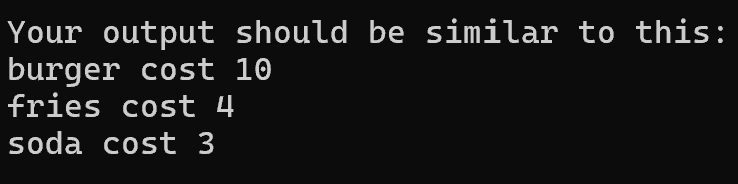
\includegraphics[scale=0.8]{./imgs/menu_output.png}
		    \end{minipage}
		\end{center}






%new_question
	\item 	
		%https://edabit.com/challenge/gDtHS9cAy8Fs2X7pH
		Write a \textbf{function} that takes a list, called $elements$, and returns a dictionary detailing how many times each element is repeated.
		
		\textbf{Examples:}  
		\begin{itemize}  
			\item count\_repetitions([\csq{cat}, \csq{dog}, \csq{cat}, \csq{cow}, \csq{cow}, \csq{cow}]) $\rightarrow$ \{ \csq{cow}: 3, \csq{cat}: 2, \csq{dog}: 1 \}
			\item count\_repetitions([1, 5, 5, 5, 12, 12, 0, 0, 0, 0, 0, 0]) $\rightarrow$ \{ 0: 6, 5: 3, 12: 2, 1: 1 \}
			\item count\_repetitions([\csq{Infinity}, \csq{null}, \csq{Infinity}, \csq{null}, \csq{null}]) $\rightarrow$ \{ \csq{null}: 3, \csq{Infinity}: 2 \}
		\end{itemize} 

%new_question
\item
	Write a \textbf{function} that takes a dictionary, called $store$, representing items and their prices, and an integer, called $wallet$, 
	representing the amount of money you have. The function should return a list of items you can afford.
	If you cannot afford anything, return an empty list.

	\textbf{Examples:}  
	\begin{itemize}  
		\item items\_purchase(\{\csq{Water}: 1, \csq{Bread}: 3, \csq{TV}: 1000\}, 300) $\rightarrow$ [\csq{Bread}, \csq{Water}]
		\item items\_purchase(\{\csq{Apple}: 4, \csq{Pan}: 100, \csq{Spoon}: 2 \}, 100) $\rightarrow$ [\csq{Apple}, \csq{Pan}, \csq{Spoon}]
		\item items\_purchase(\{\csq{Phone}: 999, \csq{Laptop}: 5000, \csq{PC}: 1200 \}, 1) $\rightarrow$ []
	\end{itemize}  

%new_question
\item
	Write a \textbf{function} that takes a dictionary, called $sales$, where the keys are product names and the values are the number of units sold. 
	The function should return the total number of products sold.

	\textbf{Examples:}  
	\begin{itemize}  
		\item total\_sales(\{\csq{Laptop}: 5, \csq{Phone}: 10, \csq{Tablet}: 3\}) $\rightarrow$ 18
		\item total\_sales(\{\csq{Shoes}: 20, \csq{Hats}: 15, \csq{Jackets}: 10\}) $\rightarrow$ 45
		\item total\_sales(\{\csq{Book}: 1, \csq{Pen}: 2, \csq{Notebook}: 1\}) $\rightarrow$ 4
	\end{itemize}

%new_question
\item
	Write a \textbf{function} that takes a dictionary, called $employee\_salaries$, where the keys are employee names and the values are their salaries. 
	The function should return a list of employees earning above a given salary.
	
	\textbf{Examples:}  
	\begin{itemize}  
		\item high\_earners(\{\csq{Alice}: 50000, \csq{Bob}: 75000, \csq{Charlie}: 100000\}, 60000) $\rightarrow$ [\csq{Bob}, \csq{Charlie}]
		\item high\_earners(\{\csq{David}: 30000, \csq{Emma}: 45000, \csq{Frank}: 50000\}, 40000) $\rightarrow$ [\csq{Emma}, \csq{Frank}]
		\item high\_earners(\{\csq{George}: 25000, \csq{Hannah}: 27000, \csq{Ian}: 29000\}, 30000) $\rightarrow$ []
	\end{itemize}


%new_question
\item
	Write a \textbf{function} that takes a dictionary, called $donations$, where the keys are donor names and the values are the amount donated. 
	The function should return the total amount donated.
	
	\textbf{Examples:}  
	\begin{itemize}  
		\item total\_donations(\{\csq{John}: 100, \csq{Sarah}: 200, \csq{Mike}: 50\}) $\rightarrow$ 350
		\item total\_donations(\{\csq{Anna}: 500, \csq{Tom}: 1000, \csq{Jerry}: 1500\}) $\rightarrow$ 3000
		\item total\_donations(\{\csq{Chris}: 25, \csq{Alex}: 30, \csq{Morgan}: 45\}) $\rightarrow$ 100
	\end{itemize}




%new_question
\item
	Write a \textbf{function} that takes a list of \textbf{fruits} and returns the total \textbf{caloric value} of the fruits consumed. You may use the following 
	dictionary named $calories$:
	\begin{center}
		\textit{calories} = \{ \csq{apple} : 95, \csq{banana} : 105, \csq{orange} : 62, 
			\csq{grape} 3, \csq{pear} : 102\}
	\end{center}
	Hint: You can calculate the total calories by summing up the caloric values of all valid 
	fruits in the list. You may assume the \textit{calories} dictionary is defined in your code.  
	You don't need to rewrite it.
	
	
	\textbf{Examples:}  
	\begin{itemize}  
		\item total\_calories([\csq{apple}, \csq{banana}, \csq{orange}]) 
			$\rightarrow$ 262 (since 95 + 105 + 62 = 262)
		\item total\_calories([\csq{grape}, \csq{grape}, \csq{grape}, \csq{grape}, \csq{grape}]) 
			$\rightarrow$ 15
		\item total\_calories([\csq{banana}, \csq{pear}, \csq{apple}]) $\rightarrow$ 302
	\end{itemize}


%new_question
\item
	Write a \textbf{function} that takes a list of \textbf{ingredients} and returns the total 
	\textbf{cost} of making a recipe. You may use the following dictionary named $prices$:
	\begin{center}
		prices = \{ \csq{flour} : 2.50, \csq{sugar} : 1.80, \csq{eggs} : 3.00, \csq{milk} : 2.00, 
			\csq{butter} : 2.75, \csq{vanilla} : 4.50, \csq{chocolate} : 5.00 \}
	\end{center}
	Hint: You can calculate the total cost by summing up the prices of all valid ingredients in 
	the list.  You may assume the \textit{prices} dictionary is defined in your code.  You don't 
	need to rewrite it.
	
	\textbf{Examples:}  
	\begin{itemize}  
		\item total\_cost([\csq{flour}, \csq{sugar}, \csq{eggs}, \csq{butter}]) $\rightarrow$ 10.05
		\item total\_cost([\csq{milk}, \csq{vanilla}, \csq{chocolate}]) $\rightarrow$ 11.50
		\item total\_cost([\csq{eggs}, \csq{eggs}, \csq{flour}, \csq{sugar}]) $\rightarrow$ 10.30
	\end{itemize}





%end_of_questions


%\item Write a program that will convert some amount of pennies into the fewest amount of dollars and coins possible.  For example, 75 pennies is 3 quarters.  86 pennies is 3 quarters, 1 dime, and 1 penny.  130 pennies is 1 dollar, 1 quarter and 1 nickel.  Let the user pick the number of pennies.  You may assume the largest input is 499 pennies.\\
%Hint: the way to do this is to always substitute for the largest denomination if available.  For example, if there is at least 100 pennies substitute for a dollar before quarters.

\end{enumerate}
\end{document}








%new_question
	%new
	\item 
		Write a \textbf{function} that takes a list of strings $delimited\_words$ and returns a dictionary.

		\textbf{Examples:}		
		\begin{itemize}
			\item  str\_to\_dict([\csq{1=one}, \csq{2=two}, \csq{3=three}, \csq{4=four}]) $\rightarrow$ {\csq{1}: \csq{one}, \csq{2}: \csq{two}, \csq{3}: \csq{three}, \csq{4}: \csq{four}}
			\item  str\_to\_dict([\csq{dog=bark}, \csq{cat=meow}, \csq{cow=moo}]) $\rightarrow$ {\csq{dog}: \csq{bark}, \csq{cat}: \csq{meow}, \csq{cow}: \csq{moo}}
			\item  str\_to\_dict([\csq{bob=human}, \csq{lola=dog}, \csq{mittens=cat}, \csq{todd=frog}]) $\rightarrow$ {\csq{bob}: \csq{human}, \csq{lola}: \csq{dog}, \csq{mittens}: \csq{cat}, \csq{todd}: \csq{frog}}
		\end{itemize}





%new_question
	%paper-based
	\item 	
		Once again, I've broken my keyboard, and the letter I type is not the same as the letter produced. Below is a table of everything that is going wrong.\\
		\begin{center}
		    \begin{minipage}{.3\textwidth}
		        \begin{tabular}{l|c}
		            \textbf{Typed letter} & \textbf{Produced letter} \\ \hline
		            e & 3 \\
		            c & k \\
		            c & v \\
		            r & u \\
		            x & y \\
		            y & x \\
		        \end{tabular}
		    \end{minipage}
		\end{center}
		Write a \textbf{function} that returns the table's typed letter and produced letter as a key-value pair.




%new_question
\item
	Write a \textbf{function} that takes a dictionary, called $fuel\_efficiency$, where the keys are car models and the values are lists of miles per gallon (MPG) 
	recorded in different driving conditions. The function should return a dictionary mapping each car model to its average MPG.

	\textbf{Examples:}  
	\begin{itemize}  
		\item average\_mpg(\{\csq{Toyota Corolla}: [30, 32, 28], \csq{Honda Civic}: [35, 37, 34]\}) $\rightarrow$ \{\csq{Toyota Corolla}: 30, \csq{Honda Civic}: 35.33\}
		\item average\_mpg(\{\csq{Tesla Model 3}: [120, 115, 125], \csq{Nissan Leaf}: [110, 112, 108]\}) $\rightarrow$ \{\csq{Tesla Model 3}: 120, \csq{Nissan Leaf}: 110\}
		\item average\_mpg(\{\csq{Chevy Malibu}: [22, 24, 23], \csq{Hyundai Sonata}: [27, 28, 29]\}) $\rightarrow$ \{\csq{Chevy Malibu}: 23, \csq{Hyundai Sonata}: 28\}
	\end{itemize}



%new_question
\item
	Write a \textbf{function} that takes a dictionary, called $school\_attendance$, where the keys are student names and the values are lists of attendance records 
	(1 for present, 0 for absent). The function should return a dictionary mapping each student to their attendance percentage.
	
	\textbf{Examples:}  
	\begin{itemize}  
		\item attendance\_average(\{\csq{Alice}: [1, 1, 0, 1], \csq{Bob}: [1, 0, 0, 1], \csq{Charlie}: [1, 1, 1, 1]\}) $\rightarrow$ \{\csq{Alice}: 0.75, \csq{Bob}: 0.5, \csq{Charlie}: 1.0\}
		\item attendance\_average(\{\csq{David}: [1, 1, 1, 0, 0], \csq{Emma}: [1, 1, 1, 1, 1], \csq{Frank}: [0, 0, 0, 0, 0]\}) $\rightarrow$ \{\csq{David}: 0.6, \csq{Emma}: 1.0, \csq{Frank}: 0.0\}
		\item attendance\_average(\{\csq{George}: [1, 1, 1, 1], \csq{Hannah}: [0, 1, 0, 1], \csq{Ian}: [1, 0, 1, 0]\}) $\rightarrow$ \{\csq{George}: 1.0, \csq{Hannah}: 0.5, \csq{Ian}: 0.5\}
	\end{itemize}


%new_question
\item
	A university wants to identify courses with high enrollments. Write a \textbf{function} that takes a dictionary, called $course\_enrollment$, 
	where the keys are course names and the values are the number of students enrolled. The function should return a list of courses with enrollments 
	above a given number.
	
	\textbf{Examples:}  
	\begin{itemize}  
		\item high\_enrollment(\{\csq{Math 101}: 150, \csq{History 202}: 80, \csq{Physics 303}: 200, \csq{English 101}: 50\}, 100) $\rightarrow$ [\csq{Math 101}, \csq{Physics 303}]
		\item high\_enrollment(\{\csq{Biology 101}: 75, \csq{Chemistry 201}: 120, \csq{Philosophy 301}: 90\}, 80) $\rightarrow$ [\csq{Chemistry 201}, \csq{Philosophy 301}]
		\item high\_enrollment(\{\csq{Art 101}: 30, \csq{Music 201}: 45, \csq{Drama 301}: 40\}, 50) $\rightarrow$ []
	\end{itemize}




%new_question
%paper-based
\item
	Write a \textbf{function} that takes a list of student $grades$ and returns the student's GPA. You may use the following dictionary named $credits$:
	\begin{center}
		credits = \{ \csq{A} : 4.0, \csq{B} : 3.0, \csq{C} : 2.0, \csq{D} 1.0, \csq{F} : 0.0\}
	\end{center}
	Hint: You can calculate the GPA by adding all the valid credit points and dividing by the number of courses.
	
	\textbf{Examples:}  
	\begin{itemize}  
		\item calculate\_gpa([\csq{A}, \csq{C}, \csq{B}, \csq{B}, \csq{A}]) $\rightarrow$ 3.2
		\item calculate\_gpa([\csq{A}, \csq{C}, \csq{A}, \csq{B}, \csq{D}]) $\rightarrow$ 2.8
		\item calculate\_gpa([\csq{B}, \csq{B}, \csq{C}, \csq{A}, \csq{F}]) $\rightarrow$ 2.6
	\end{itemize}




%new_question
\item
	Write a \textbf{function} that takes a list of strings $words$ and returns a dictionary where the keys are word lengths and the values are lists of words with that length.
	
	\textbf{Examples:}  
	\begin{itemize}  
		\item group\_words\_by\_length([\csq{apple}, \csq{banana}, \csq{cat}, \csq{dog}, \csq{elephant}, \csq{fox}, \csq{hat}, \csq{iguana}])  
		$\rightarrow$ \{5: [\csq{apple}], 6: [\csq{banana}, \csq{iguana}], 3: [\csq{cat}, \csq{dog}, \csq{fox}, \csq{hat}], 8: [\csq{elephant}]\}\\
		\item group\_words\_by\_length([\csq{table}, \csq{chair}, \csq{pen}, \csq{pencil}, \csq{notebook}, \csq{book}]) 
		$\rightarrow$ \{5: [\csq{table}, \csq{chair}], 3: [\csq{pen}], 6: [\csq{pencil}], 8: [\csq{notebook}], 4: [\csq{book}]\}\\
		\item group\_words\_by\_length([\csq{hi}, \csq{hello}, \csq{bye}, \csq{goodbye}]) 
		$\rightarrow$ \{2: [\csq{hi}], 5: [\csq{hello}], 3: [\csq{bye}], 7: [\csq{goodbye}]\}
	\end{itemize}


%new_question
\item
	Write a \textbf{function} that takes a list of integers $numbers$ and returns a dictionary where the keys are \csq{odd} and \csq{even}, and the values are lists of 
	numbers that fall into each category.
	
	\textbf{Examples:}  
	\begin{itemize}  
		\item group\_by\_parity([1, 2, 3, 4, 5, 6, 7, 8, 9, 10]) $\rightarrow$ \{\csq{odd}: [1, 3, 5, 7, 9], \csq{even}: [2, 4, 6, 8, 10]\}
		\item group\_by\_parity([12, 15, 18, 21, 24, 27]) $\rightarrow$ \{\csq{odd}: [15, 21, 27], \csq{even}: [12, 18, 24]\}
		\item group\_by\_parity([7, 13, 19, 25]) $\rightarrow$ \{\csq{odd}: [7, 13, 19, 25], \csq{even}: []\}
	\end{itemize}

%new_question
\item
	Write a \textbf{function} that takes a list of integers $numbers$ and returns a dictionary where the keys represent number ranges (\csq{low}, \csq{medium}, \csq{high}) 
	and the values are lists of numbers that fall into those categories.  

	The number ranges are defined as follows:
	\begin{enumerate}  
		\item \csq{Low} contains numbers less than 10.  
		\item \csq{Medium} contains numbers between 10 and 50 (inclusive).  
		\item \csq{High} contains numbers greater than 50.  
	\end{enumerate}  
	
	\textbf{Examples:}  
	\begin{itemize}  
		\item group\_by\_range([3, 12, 25, 7, 55, 80, 42]) $\rightarrow$ \{\csq{low}: [3, 7], \csq{medium}: [12, 25, 42], \csq{high}: [55, 80]\}
		\item group\_by\_range([5, 15, 30, 60, 75, 90]) $\rightarrow$ \{\csq{low}: [5], \csq{medium}: [15, 30], \csq{high}: [60, 75, 90]\}
		\item group\_by\_range([1, 2, 3, 4, 5]) $\rightarrow$ \{\csq{low}: [1, 2, 3, 4, 5], \csq{medium}: [], \csq{high}: []\}
	\end{itemize}


%new_question
\item
Write a \textbf{function} that takes a list of words $words$ and returns a dictionary where the keys categorize words based on the presence of numerical digits.  
	The categories are defined as follows:
	\begin{enumerate}  
		\item \csq{Contains digits} includes words that have at least one numerical digit (0-9).  
		\item \csq{No digits} includes words that contain only alphabetic characters.  
	\end{enumerate}  
	
	\textbf{Examples:}  
	\begin{itemize}  
		\item words\_by\_digits([\csq{hello}, \csq{world123}, \csq{python}, \csq{code2024}]) $\rightarrow$ \{\csq{contains digits}: [\csq{world123}, \csq{code2024}], \csq{no digits}: [\csq{hello}, \csq{python}]\}
		\item words\_by\_digits([\csq{abc}, \csq{xyz}, \csq{data}, \csq{42days}, \csq{7up}]) $\rightarrow$ \{\csq{contains digits}: [\csq{42days}, \csq{7up}], \csq{no digits}: [\csq{abc}, \csq{xyz}, \csq{data}]\}
		\item words\_by\_digits([\csq{one}, \csq{two}, \csq{three}]) $\rightarrow$ \{\csq{contains digits}: [], \csq{no digits}: [\csq{one}, \csq{two}, \csq{three}]\}
	\end{itemize}

%new_question
\item
	Write a \textbf{function} that takes a list of words $words$ and returns a dictionary where the keys categorize words based on whether they are palindromes.  
	The categories are defined as follows:
	\begin{enumerate}  
		\item \csq{Palindrome} includes words that read the same forward and backward.  
		\item \csq{Non-palindrome} includes all other words.  
	\end{enumerate}  
	
	\textbf{Examples:}  
	\begin{itemize}  
		\item palindromes([\csq{madam}, \csq{racecar}, \csq{hello}, \csq{level}, \csq{python}]) $\rightarrow$ \{\csq{palindrome}: [\csq{madam}, \csq{racecar}, \csq{level}], \csq{non-palindrome}: [\csq{hello}, \csq{python}]\}
		\item palindromes([\csq{noon}, \csq{civic}, \csq{deed}, \csq{open}, \csq{loop}]) $\rightarrow$ \{\csq{palindrome}: [\csq{noon}, \csq{civic}, \csq{deed}], \csq{non-palindrome}: [\csq{open}, \csq{loop}]\}
		\item palindromes([\csq{apple}, \csq{banana}, \csq{cherry}]) $\rightarrow$ \{\csq{palindrome}: [], \csq{non-palindrome}: [\csq{apple}, \csq{banana}, \csq{cherry}]\}
	\end{itemize}


%new_question
\item
	Write a \textbf{function} that takes a list of words $words$ and returns a dictionary where the keys categorize words based on whether they start and end with the same letter.  
	The categories are defined as follows:
	\begin{enumerate}  
		\item \csq{Same start and end} includes words where the first and last letter are the same.  
		\item \csq{Different start and end} includes words where the first and last letter are different.  
	\end{enumerate}  
	
	\textbf{Examples:}  
	\begin{itemize}  
		\item words\_by\_start\_end([\csq{radar}, \csq{apple}, \csq{civic}, \csq{banana}, \csq{level}]) $\rightarrow$ \{\csq{same start and end}: [\csq{radar}, \csq{civic}, \csq{level}], \csq{different start and end}: [\csq{apple}, \csq{banana}]\}
		\item words\_by\_start\_end([\csq{hello}, \csq{world}, \csq{refer}, \csq{test}, \csq{wow}]) $\rightarrow$ \{\csq{same start and end}: [\csq{refer}, \csq{wow}], \csq{different start and end}: [\csq{hello}, \csq{world}, \csq{test}]\}
		\item words\_by\_start\_end([\csq{a}, \csq{b}, \csq{c}]) $\rightarrow$ \{\csq{same start and end}: [\csq{a}, \csq{b}, \csq{c}], \csq{different start and end}: []\}
	\end{itemize}
